\chapter{Bottlenecks of Metal Sulfide Solar Cells}

\section{Promising Candidate Solar Absorber Materials}
Refer to: CH 5 (other PV materials) + pg 187 (future of PV) \cite{PV_Goetzberger}\\

As already discussed, to make solar energy generation on a large scale economically viable, it must be possible to make devices with an LCOE that is comparable to fossil-fuel resources. Furthermore, the materials that make up the devices must also be sufficiently abundant such that there would be enough to make a substantial number of devices in the first place. For this reason there is a drive for photovoltaic materials that could be made using the lost-cost methods associated with second-generation technology, but containing only earth-abundant components. Gauging the abundance of a given material is not as trivial a process as looking at crustal abundance as supply, demand, geographical distribution and extraction must all be considered. However, knowledge of solar cell technologies made from various different materials opens up the possibility of utilizing multiple different materials to collectively contribute to the global solar power capacity to enable larger-scale power generation from this renewable, low-carbon resource. Additionally by studying various different materials, the scientific community could eventually discover a select few that have the best properties to enable low-cost synthesis of highly efficient devices to eventually significantly reduce the LCOE of solar power.\\

Currently, Cu$_2$ZnSnS$_4$ (CZTS) is one of the most studied candidate earth-abundant thin-film solar cell materials \cite{CZTS_vs_MAPI}. The potential of CZTS for photovoltaic applications was realised in 1988 by Ito and Nakazawa \cite{first_CZTS}. The band gap of the material has been predicted \cite{CZTS_bandgap_theory} and measured \cite{CZTS_bandgap_exp} to be 1.5 eV, which corresponds to a theoretical conversion efficiency limit of 28\% as predicted by Shockley-Quiesser \cite{SQ_1961}. However, the current record device efficiency is 8.8\% \cite{CZTS_record} and it is believed that this figure must be increased to at least 15\% for the devices to be commercially viable \cite{SS}. PV devices composed of a CZTS absorber layer are hampered by low open circuit voltage (V$_{OC}$) \cite{SS}, which is believed to be due to the formation of secondary phases \cite{CZTS_phases} and defects \cite{CZTS_defects} in CZTS, although the exact origin of the low V$_{OC}$ remains unknown. The first component of this study is therefore an attempt to determine possible origins of this deficit in CZTS.\\

%MAPbI$_3$ is an example of a hybrid halide perovskite solar cell material, which are regarded as a convergence of inorganic thin-film and dye-sensitised solar cells (DSSC's) \cite{Federico}. Research on such materials dates back to 1928 \cite{Jarv_7}. The efficiency of MAPbI$_3$ solar cells however has increased rapidly between 2009 and 2014 from 3.8\% for MAPbI$_3$-based DSSC's to 20.1\% for a planar MAPbI$_3$-based thin-film solar cells \cite{CZTS_vs_MAPI} and has therefore surpassed the record efficiency of both conventional DSSC's as well as the earth-abundant thin-film PV absorber material CZTS \cite{Federico}. Electricity generation in a typical PV device, such as that shown in the schematic in figure \ref{PV_schematic}, is dependent upon charge separation by variation in material composition, as in a p-n junction. However, in ferroelectric materials charge separation can also be achieved due to the intrinsic crystal field in a homogeneous material. The crystal polarity creates microscopic electric fields across domains, separating photogenerated excitons into free charges, and segregating the transport of the free charges to reduce recombination rates \cite{keith}. Hybrid perovskites have been shown to exhibit spontaneous electric polarization \cite{Jarv}.
%Therefore, one possible explanation for the high efficiency of MAPbI$_3$-based solar cells is enhanced separation of photoexcited electron and hole pairs, and hence reduced rate of electron-hole recombination, due to the presence of ferroelectric domains \cite{Jarv, Federico}. Although the stability of MAPbI$_3$-based solar cells has been identified as a big challenge for these devices, as CH$_3$NH$_3$PbI$_3$ is very sensitive to polar solvents such as water and so readily dissolves and decomposes into PbI$_2$ \cite{MAPI}. \\

A number of interesting PV phenomena have been observed in ferroelectric (FE) materials  such as the bulk photovoltaic effect (BPE) and the anomalous photovoltaic effect (APE) \cite{keith}. Ferroelectric materials usually have a high dielectric constant (which was mentioned in section \ref{PV_properties} as an important parameter for a photovoltaic material) and they possess a spontaneous electric polarization that can be switched between two or more states using an electric field \cite{new_FE_PV_1}.
The BPE was first recorded in 1956 in BaTiO$_3$ \cite{keith_46}, where photovoltages were measured in un-doped single crystals \cite{keith}.
The BPE effect is distinctly different from the typical PV effect in semiconductor
p-n junctions as it is the polarization electric field that is the driving force for the photocurrent in FE-PV devices \cite{FE_PV_rev1}. 
The APE was first observed in PbS films in 1946 \cite{keith_54} and has since been reported in polycrystalline CdTe, ZnTe, InP \cite{keith_55, keith_56, keith_57}, where photovoltages output along the polarization direction can be significantly larger than the band gap of the material \cite{FE_PV_rev1}, which is usually the limit for a semiconductor PV material \cite{keith}. 
The Shockley-Queisser limit, which prevents any single p-n junction solar cell from converting more than 33.7\% of the incident light into electricity, has not been predicted to apply for these photovoltaic phenomena. An upper limit for the theoretical power conversion efficiency (PCE) from this photovoltaic mechanism seems to still be an open question \cite{new_FE_PV}, although an ultimate maximum efficiency of any single-band gap absorber of 44\% has been set by thermodynamic considerations \cite{SQ_1961}.\\ %Theories to explain the PV phenomena observed in FE materials are discussed further in section \ref{FE_PV_section}.\\

The identification and understanding of such phenomena may open up the possibility of more efficient PV devices constructed from a number of different photoferroelectric materials. However, most of the commonly used ferroelectric materials such as LiNbO$_3$ and BaTiO$_3$ have band gaps larger than 3 eV and can therefore only absorb sunlight in the UV range to convert into electricity, which accounts for only around 3.5\% of the solar spectrum \cite{FE_PV_rev1}, which is illustrated in figure \ref{solar_spectrum}. The optimal range for the band gap in order to absorb the majority of the solar spectrum under typical radiation conditions is between 1.06 eV and 1.50 eV \cite{CZTS_book}. Research efforts have also gone into adjusting the optical absorption of ferroelectric materials without influencing the ferroelectric properties of the material through chemical doping or alloying \cite{FE_PV_rev1}. In Bi$_4$Ti$_3$O$_{12}$ (BiT) the optical band gap has been tuned in such a way, resulting in a decrease from 3.6 eV to 2.7 eV \cite{FE_PV_rev1_83}, although this is still considerably larger than the optimal range for a PV absorber material.\\

This then leads on to the second component of this study, which is an investigation of the optoelectronic properties of new candidate solar absorber materials that may also exhibit ferroelectricity, but have band gaps within the optimal range for the absorption of sunlight. 
In theory, these materials 
%may exhibit the exceptionally high performance of MAPbI$_3$-based solar cells (ideally without the instability issues suffered by MAPbI$_3$) or 
enable the possibility of exploiting novel photovoltaic phenomena such as the anomalous and bulk photovoltaic effects to overcome the Shockley-Quiesser efficiency limit without the need for such complicated device architectures as in third-generation tandem solar cells. Although the difference between the Shockley-Quiesser limit and the ultimate thermodynamic limit of a solar material is not enormous, it is also possible that ferroelectric materials have properties that enable more efficient devices to be made more easily, such as good screening of the effect of defects due to a high dielectric constant or enhanced electron-hole separation from ferroelectric domains resulting in reduced recombination and a higher performance solar cell with `low quality' defective and nanostructured materials. Such technologies could provide one possible route for the technological breakthrough that could enable economically-viable, large-scale solar energy generation.

\section{Possible Performance Bottlenecks of {\CZTS } Devices}
** Check against Laurie's April highlights (top two bullet points on disorder) + Susan Siebentritt's: Why are kesterite solar cells not 20 percentage efficient?\\

\begin{figure}[h!]
  \centering
    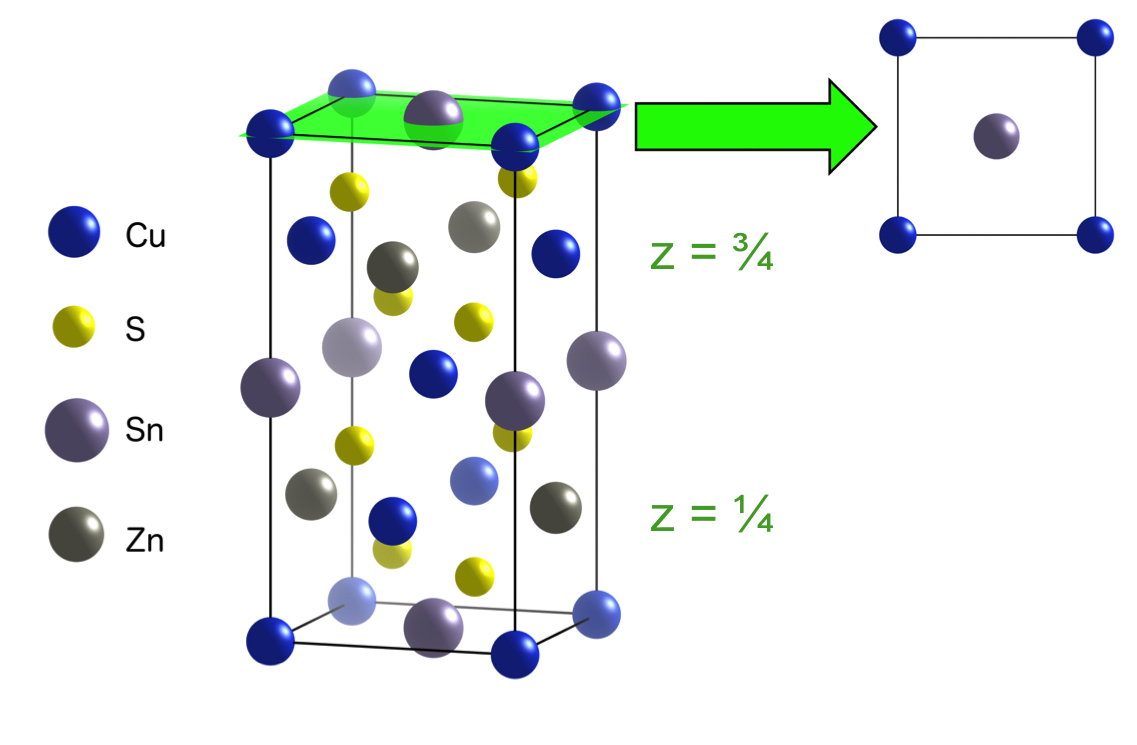
\includegraphics[width=0.7\textwidth]{figures/CZTS_cell.png}
    \caption{The conventional unit cell of CZTS (Cu$_{2}$ZnSnS$_{4}$) with the ground-state kesterite crystal structure (space group $I\bar{4}$). The structure consists of alternating layers of Cu-Sn and Cu-Zn where Cu-Zn layers are at z=$\frac{1}{4}$ and z=$\frac{3}{4}$.}
  \label{CZTS_cell}
\end{figure}

The ground state crystal structure of CZTS (Cu$_{2}$ZnSnS$_{4}$) is kesterite (space group $I\bar{4}$). The conventional unit cell of CZTS is shown in figure \ref{CZTS_cell}, where each S is surrounded by two Cu, one Zn, and one Sn to satisfy local charge neutrality and the valence-octet rule.
Kesterites meet two necessary conditions for highly efficient solar cells, which are a band gap that is both direct and relatively well-matched to the solar spectrum \cite{CZTS_book}.
Over the last decade the power conversion efficiency of PV devices based on kesterite, Cu$_2$ZnSn(S$_x$Se$_{1-x}$)$_4$ (CZTSSe), compounds has improved greatly from around 5\% in 2004 to 12.6\% in 2013 \cite{culprit_2}. However, this is still far from the record efficiencies of Cu(In$_{1-y}$,Ga$_y$)Se$_2$ (CIGSe) devices of $>$20\%, where the materials have very similar band gaps to those of CZTSSe \cite{culprit} and so should have the same theoretical efficiency limit as predicted by Shockley and Queisser \cite{SQ_1961}. Furthermore, the rate of improvement seems to have slowed considerably recently with the last improvement in efficiency being reported in 2014 and with only a 0.1\% improvement \cite{culprit_3}. A large number of possible explanations have been proposed to explain the current difference in efficiency between CZTSSe and CIGSe devices, many of these are illustrated in figure \ref{kesterite_bottlenecks}. The majority of studies converge towards the low open circuit voltage (V$_{OC}$) relative to the band gap, i.e. the V$_{OC}$ deficit, being the main limiting factor on device performance. As can be seen from the position of CZTSSe devices on the plot in figure \ref{Voc}, the open circuit voltages measured for these devices are considerably less than that of a CIGS device, which has a similar value for the band gap of the material.\\

\begin{figure}[h!]
  \centering
    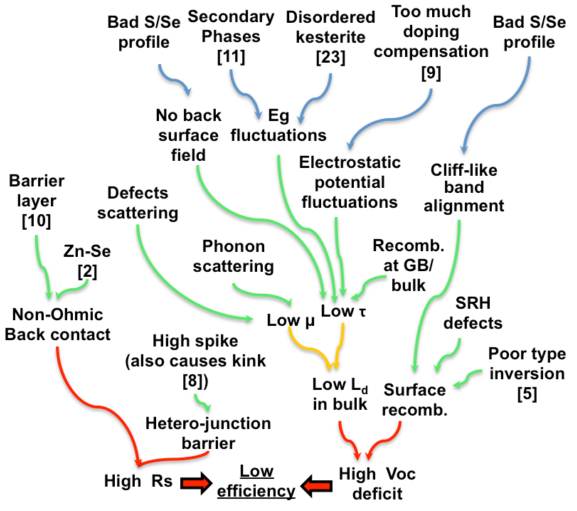
\includegraphics[width=0.75\textwidth]{figures/kesterite_bottlenecks.png}
    \caption{Mapping of the numerous possible mechanisms limiting the efficiency in kesterite devices and their possible causes. R$_s$ is the series resistance between the absorber layer and back contact of the device and V$_{OC}$ is the open circuit voltage across the absorber layer. Figure take from \citenum{CZTS_scale_up}.}
  \label{kesterite_bottlenecks}
\end{figure}

\begin{figure}[h!]
  \centering
    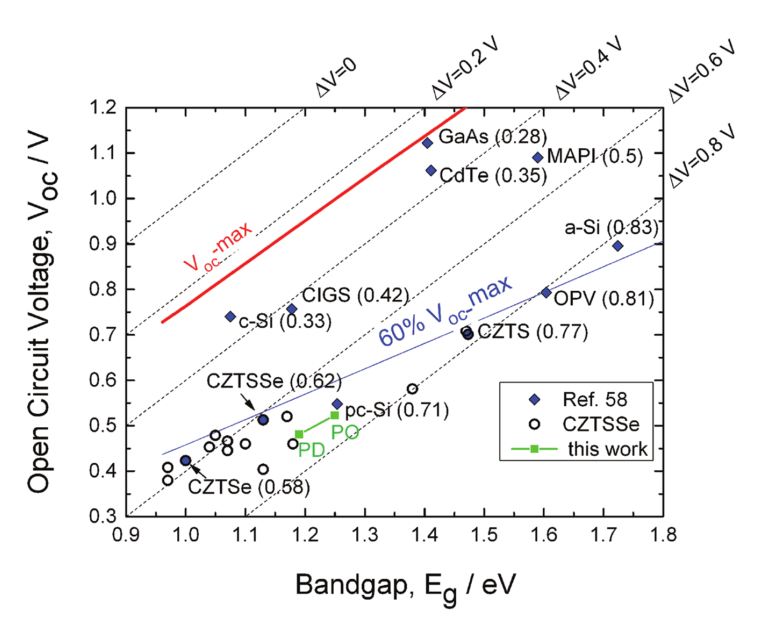
\includegraphics[width=0.85\textwidth]{figures/Voc.png}
    \caption{V$_{OC}$ versus band gap of high performance CZTSSe devices ($>$9\% efficiency) indicated by circles with best devices based on other photovoltaic materials shown for comparison by diamond symbols: Methyl-ammonium lead iodide (MAPI), amorphous silicon (a-Si), organic photovoltaic films (OPV), crystalline silicon (c-Si) and polycrystalline silicon (pc-Si). The oblique lines give a constant V$_{OC}$ deficit from 0.8 V to 0 V. The green points correspond to CZTSSe films that are partially ordered (PO) or partially disordered (PD) due to disorder amongst Cu and Zn. Figure take from reference \citenum{culprit}.}
  \label{Voc}
\end{figure}

As figure \ref{kesterite_bottlenecks} shows, there are many different possible causes of the  V$_{OC}$ deficit in kesterite solar cells. Developing fabrication techniques to reduce the deficit is therefore an even greater challenge when the exact cause is not yet known.
This is an area in which computational materials simulations should be able to provide valuable insight to help pinpoint the specific sources of the V$_{OC}$ deficit in kesterite solar cells. The true power of simulation is the ability to take a perfect system and introduce various imperfections one and a time and then study the effect that particular imperfection could have on device performance. As opposed to in a real system in which there is a myriad of possible causes for each observation, as illustrated in figure \ref{kesterite_bottlenecks}.
In our simulations we will start from the most simple system possible, before making any attempts to build up in complexity. Devices made from a compound of \CZTS  and Cu$_2$ZnSnSe$_4$, i.e. Cu$_2$ZnSn(S$_x$Se$_{1-x}$)$_4$, so far have given the highest performance devices, however in this study we are currently focusing on just the pure selenide material, CZTS. In addition to simplifying the system, figure \ref{Voc} also indicates that the V$_{OC}$ deficit is worse in purely CZTS devices and so potentially studying causes of the problem in this particular system could be more informative. Also although ultimately the aim is to make thin-film devices from CZTS, in which the material is likely to be highly polycrystalline with many grain boundaries, we are currently just focusing on the bulk material. We are doing this for two reasons. Firstly to improve the understanding of the fundamental material properties before attempting to understand a more complex system to ensure we start from a solid foundation. Secondly, it has been proposed that the V$_{OC}$ deficit in CZTSSe devices could actually be largely due to the natural bulk properties of the crystal \cite{culprit_5}. For the purposes of our study therefore measurements performed on single crystals will be the most directly relatable to our findings, wherever the data is available.\\

\begin{figure}[h!]
  \centering
    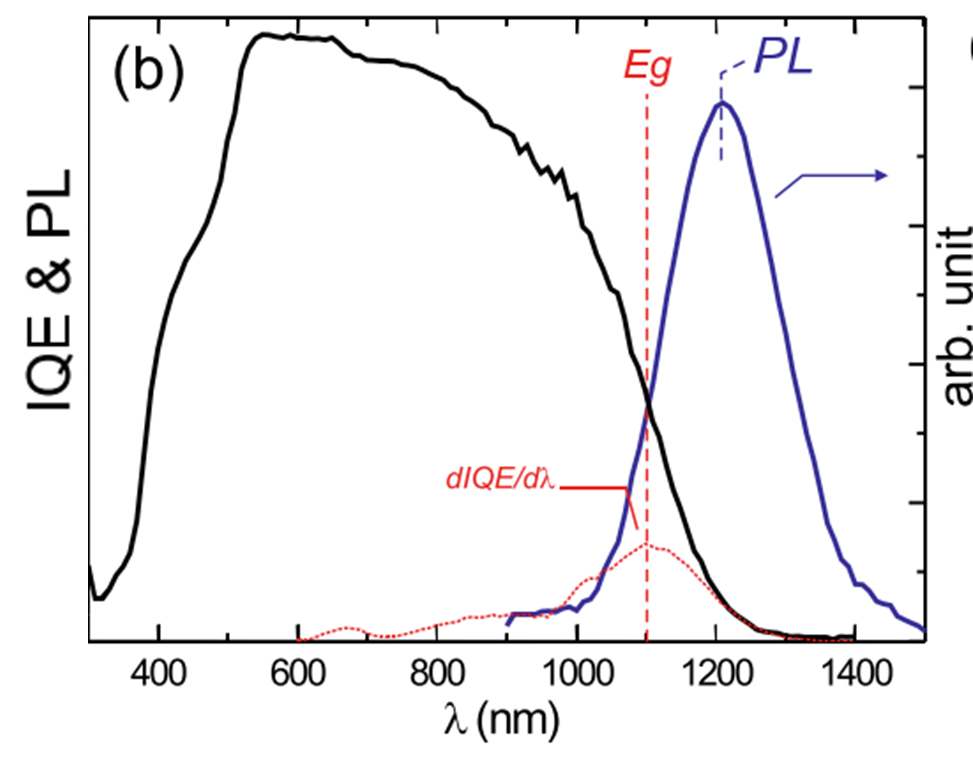
\includegraphics[width=0.7\textwidth]{figures/CZTS_PL.png}
    \caption{Internal quantum efficiency (IQE) and photoluminescence (PL) spectra of CZTSSe thin-films showing the shift of the PL peak to energies below the band gap of the material. Figure take from reference \citenum{band_tail}.}
  \label{CZTS_PL}
\end{figure}

\begin{figure}[h!]
  \centering
    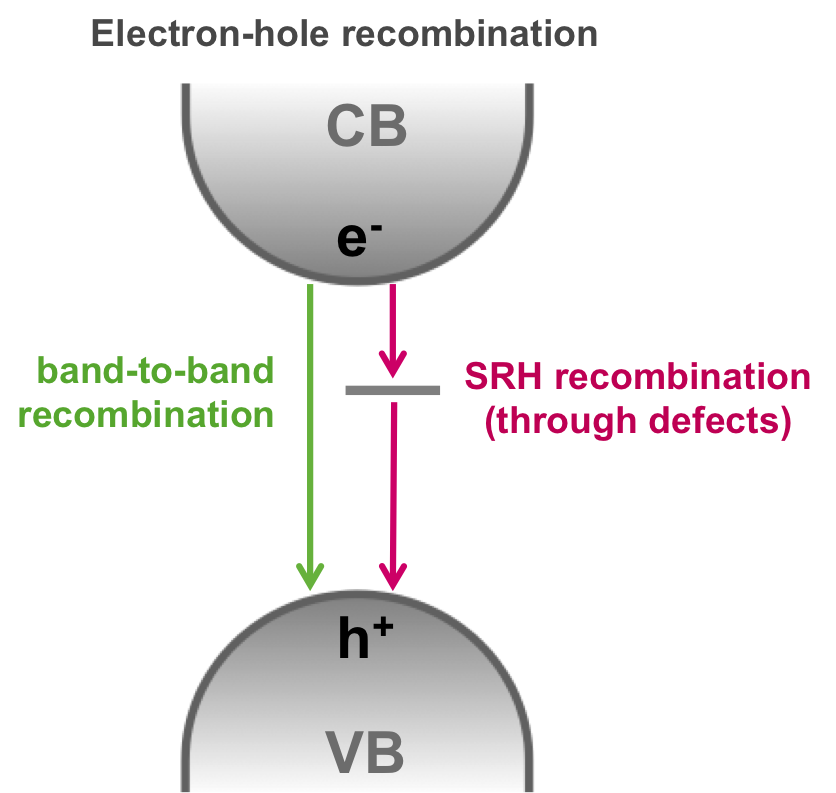
\includegraphics[width=0.45\textwidth]{figures/SRH.png}
    \caption{Illustration of Shockley-Read-Hall (SRH) electron-hole recombination due to energy states introduced into the band gap by defects.}
  \label{SRH}
\end{figure}

In general, the main cause of V$_{OC}$ deficit in a PV device is the recombination of photogenerated charge carriers in the bulk material or at surfaces \cite{culprit}. 
Figure \ref{CZTS_PL} shows photoluminescence (PL) spectroscopy measurements performed on CZTSSe thin films by Gokmen et al \cite{band_tail}. The emission spectra of semiconductors is discussed much more thoroughly in section \ref{PL_section} and a review of various PL studies performed on kesterite thin films and crystals is given in section \ref{CZTS_PL_section}, but for current purposes the key observation to be made from figure \ref{CZTS_PL} is that there is a shift in the PL peak to lower energies (red-shifting), below the value of the band gap obtained from internal quantum efficiency (IQE) measurements performed on the same thin films. It is also noted in this study when comparing the PL spectra of CZTSSe films to that of CIGSSe films that the PL peak for CZTSSe thin films is broader and that the red-shifting was roughly twice as severe. This effect is referred to as `band-edge tailing', where photons of energies less than the band gap of the material are emitted following photoexcitation and subsequent relaxation back to the ground state. This effect is known to be detrimental for device performance as emitted photons may then not have sufficient energy for subsequent photoexcitations in the absorber layer, the energy of the original photon may then not be converted into electricity if the photoexcited electron-hole pair recombine before the charge is collected \cite{Nelson4}. Band tailing and the possible causes of this detrimental effect are discussed further in section \ref{defects_in_PV}, but for now it is worth briefly noting that possible causes are: Shockley-Read-Hall recombination due to defect-induced mid-gap states \cite{SRH}, as illustrated in figure \ref{SRH}, as well as fluctuations in electrostatic potential due to the presence of charged defects and fluctuations in the band gap of the material due to an inhomogeneous composition \cite{band_tail}, which are both shown in figure \ref{band_tail_fig}.\\

\begin{figure}[h!]
  \centering
    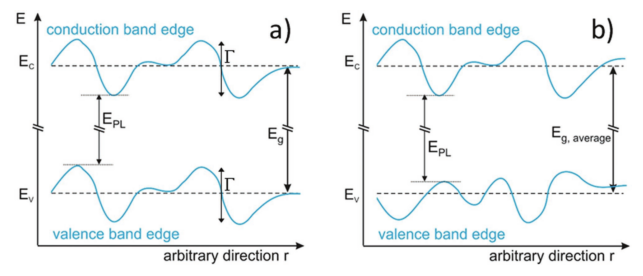
\includegraphics[width=0.9\textwidth]{figures/band_tail_fig.png}
    \caption{The effect of electrostatic potential fluctuations (a) and band gap fluctuations (b) on the electronic bands of a semiconductor. In both cases radiative transitions at energies below the (average) band gap are possible. The band gap in a is constant and not affected by local charged defects, while band edges in b can differ depending on e.g., long range composition variations. Figure taken from reference \citenum{culprit}.}
  \label{band_tail_fig}
\end{figure}

The extent of band tailing due to the additional energy levels introduced into the band gap of a material by particular intrinsic defects is dependent upon the concentration of those particular defects. The equilibrium defect concentration can be obtained directly from the defect formation energy \cite{DFT_in_mat}, which is discussed further in section \ref{defect_sections}. For materials such as CZTSSe that are still at a fairly early stage of development, theoretical predictions of defect formation energies may be the only values available to help identify specific defects and their properties in real systems \cite{kosyak}. Theoretical predictions for the formation energies and depth of defect-induced energy levels for various intrinsic point defects and defect clusters in CZTS made by Chen et al \cite{defect1} are shown in figures \ref{Chen_pt1}, \ref{Chen_pt2}, \ref{Chen_cluster1} and \ref{Chen_cluster2}. Based on the predictions made by Chen et al, figure \ref{Chen_pt2} shows that many of the intrinsic defects involving Sn would induce a mid-gap state, however figure \ref{Chen_pt1} shows that the formation energy of those particular defects would all be expected to be high. It therefore would be expected that these defects are less likely to form and should be present in lower concentrations than other defects. Although other works have suggested that the formation of this defect could be more likely if it is forms part of a particular defect cluster \cite{CZTS_n-type, culprit}. From the work by Chen on defect clusters, it is also expected that certain charge compensated defect clusters would have very low formation energies, in particular the $[Cu_{Zn}^{-} + Zn_{Cu}^{+}]$ antisite defect pair, as shown in figure \ref{Chen_cluster1}.\\

Disorder amongst Cu and Zn ions (or equivalently the formation of the $[Cu_{Zn}^{-} + Zn_{Cu}^{+}]$ antisite defect pair) in CZTS has been proposed as one possible origin of the V$_{OC}$ deficit in CZTS and consequently a number of experimental studies have been conducted to investigate this \cite{Scragg, pot_fluc_4, neutron, Schorr}. Additionally it is worth noting that this substitutional disorder does not exist in the crystal structure of CIGSe due to the considerably larger chemical mismatch between Cu with In or Ga \cite{culprit}, whereas Cu and Zn are so similar that disorder between the two species can be difficult to detect experimentally. 
As Cu and Zn are neighbouring elements in the periodic table, the changes in the bonding between the two are subtle \cite{pot_fluc}. This results in a theoretical energy difference between the two structures of just 3 meV per atom \cite{Chen2009} allowing for intermixing of the Cu and Zn cations in CZTS, which has been confirmed by neutron diffraction \cite{pot_fluc_4, neutron} and also measured using near resonant raman scattering \cite{Scragg}. However, a recent work prepared samples with varying degrees of Cu-Zn disorder (by varying the cooling rate during synthesis, which had been shown in a previous study to have a considerable effect on Cu-Zn ordering in CZTS \cite{Scragg}) and in this work they showed that a reduction in Cu-Zn order resulted in a reduction in both the band gap and V$_{OC}$, thereby not influencing the V$_{OC}$ deficit relative to the band gap of the material \cite{culprit}.

\begin{figure}[h!]
  \centering
    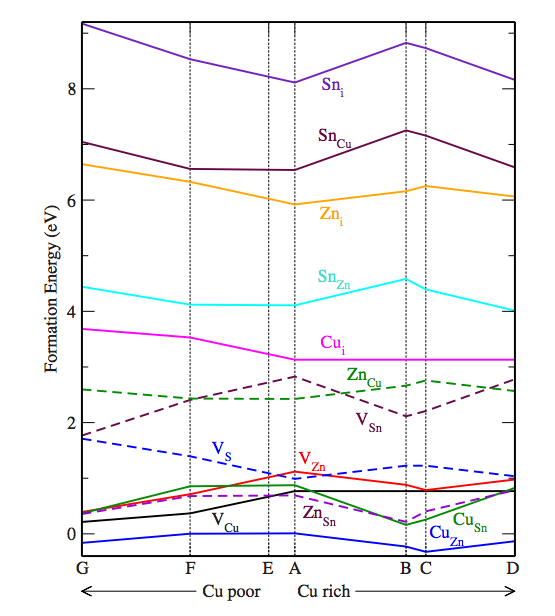
\includegraphics[width=0.8\textwidth]{figures/Chen_pt_formE.png}
    \caption{The formation energy of neutral intrinsic defects in \CZTS as a function of the chemical potential. Figure taken from reference \citenum{defect1}.}
  \label{Chen_pt1}
\end{figure}

\begin{figure}[h!]
  \centering
    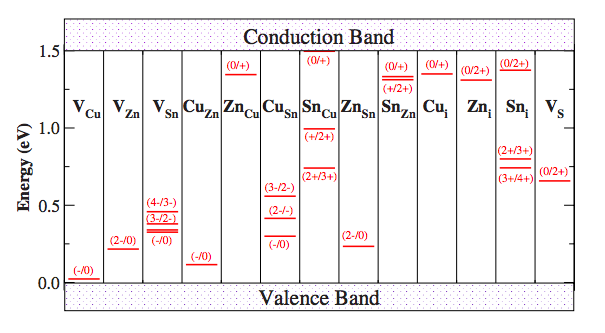
\includegraphics[width=0.8\textwidth]{figures/Chen_pt_E-level.png}
    \caption{The transition-energy levels of intrinsic defects in the band gap of \CZTS where the GGA band gap has been corrected to the experimental value 1.5 eV, and the donor levels are shifted together with the conduction band minimum (CBM) level. Figure taken from reference \citenum{defect1}.}
  \label{Chen_pt2}
\end{figure}

\begin{figure}[h!]
  \centering
    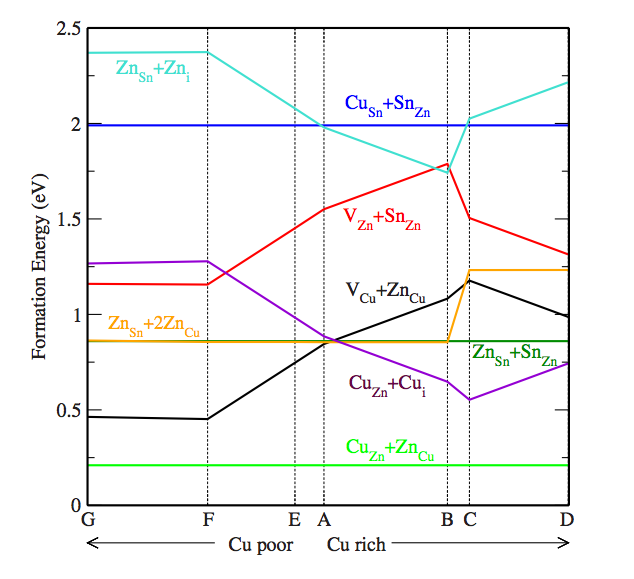
\includegraphics[width=0.8\textwidth]{figures/Chen_cluster_formE.png}
    \caption{The formation energy of charge compensated defect complexes in \CZTS as a function of the chemical potential. Figure taken from reference \citenum{defect1}.}
  \label{Chen_cluster1}
\end{figure}

\begin{figure}[h!]
  \centering
    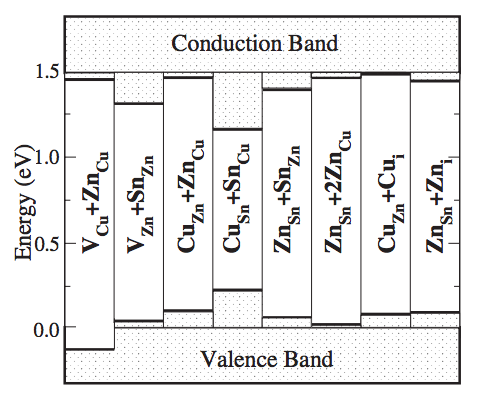
\includegraphics[width=0.7\textwidth]{figures/Chen_cluster_E-level.png}
    \caption{The conduction band minimum (CBM) and valence band maximum (VBM) levels in eV of \CZTS with different charge-compensated defect complexes relative to the host material at 0 eV and 1.5 eV respectively. Figure taken from reference \citenum{defect1}. }
  \label{Chen_cluster2}
\end{figure}

In this work we begin three investigations to explore some of the possible explanations for the V$_{OC}$ deficit in CZTS solar cells and to attempt to explain the PL spectra of CZTS shown in figure \ref{CZTS_PL}. 
As discussed above, intrinsic defects can introduce additional energy levels into the band gap of the material and energy states within the band gap are Shockley-Read-Hall recombination sites \cite{SRH}.
We re-investigate the formation energy of sulfur vacancies (V$_S$) in CZTS. This is another possible deep donor defect in CZTS and it was proposed in a recent study using admittance spectroscopy measurements performed on CZTSSe, combined with electrical modelling, that in addition to majority p-type defects in CZTSSe (giving the material its p-type conductivity), there may also been deep n-types defects \cite{CZTS_n-type}.
V$_S$ in CZTS has been predicted to produce a mid-gap state in the band gap of the material \cite{defect1}, which could provide one explanation for the poor device performance. However in the same work this particular point defect was also predicted to have a high formation energy relative to other possible intrinsic defects, making it less likely to form. However, it is possible that the formation energy of this defect is reduced when considering the typical annealing conditions of CZTS in which S is in the gaseous phase. We therefore calculate the formation energy of a V$_S$ in CZTS as a function of the sulfur chemical potential, which has been calculated as a function of temperature and pressure in a previous study \cite{Adam_sulfur}, making it possible for us to compare directly to experimental synthesis conditions.\\

Secondly, we examine possible causes of band gap broadening, which has been observed in electromodulation (??) measurements performed on CZTS crystals \cite{PVTEAM_paper}. We use materials modelling to determine the intrinsic band gap broadening to be expected even in perfect, bulk CZTS due to thermal lattice expansions. This contribution can then be subtracted from band gap broadening measured experimentally to determine how much of this effect is due to disorder and other factors. 
Lastly, we simulate thermodynamic substitution amongst Cu and Zn ions in CZTS and study the resulting changes in the distribution of electrostatic potential in the system in an attempt to extract the contribution of this particular type of disorder to the strong band tailing that has been observed in kesterite devices, which has been suggested to be due to fluctuations in electrostatic potential \cite{band_tail}.
As discussed above, disorder amongst Cu and Zn ions has not only be predicted to be very likely based on energetics but has also been observed experimentally, it would therefore be important to know if this particular type of disorder is having a detrimental effect on device performance or to at least eliminate it from the list of many possible causes of the V$_{OC}$ deficit.\\
**Edit last paragraph once PVTEAM paper published so have more info + put eris study first to match order of results?**\\

Introduce PVTEAM collaboration here?
 


\section{Predicting the Properties of New Candidate Solar Absorber Materials}
*Add explanation of investigating new materials in case bottlenecks of CZTS are unavoidable\\

The second part of this study involves using materials modelling to predict the optoelectronic properties of materials that could have the potential to be used to produce high performance PV devices, but until now have received little research interest for applications in PV.  The central idea in selecting these candidate materials was to identify any that may be ferroelectric and so could exhibit some of the novel FE-PV phenomena discussed earlier but may also have a band gap within the optimal range for solar absorption. Photoferroelectric, or photoferroic, is the name given to materials that exhibit such properties. 
Using very simple screening criteria, we identified three candidate photoferroelectric solar absorber materials from a data set of over 200 naturally occurring minerals. 
A dark-coloured material suggests (but does not guarantee) that it absorbs light in the visible range. Ferroelectric materials are a subset of materials with polar crystal structures, therefore not all polar materials exhibit ferroelectricity. It is only polar materials that also possess a spontaneous electric dipole moment within the unit cell which can be inverted by the application of an external electric field that exhibit ferroelectricity \cite{FE_subset}. 
Therefore, the conditions used to screen for candidate photoferroelectric materials shown in the Venn diagram in figure \ref{vd} are necessary conditions for photoferroelectricity, but cannot guarantee this property as a polar space group is a necessary but not sufficient condition for ferroelectricity.
The three candidate photoferroelectric materials identified by our screening process were: enargite (\enargite), stephanite (\stephanite) and bournonite (\bournonite). All three minerals are sulfosalts, which are materials that contain two or more metals, semi-metals such as antimony and arsenic, and sulfur \cite{DK}. \\

\begin{figure}[h!]
  \centering
    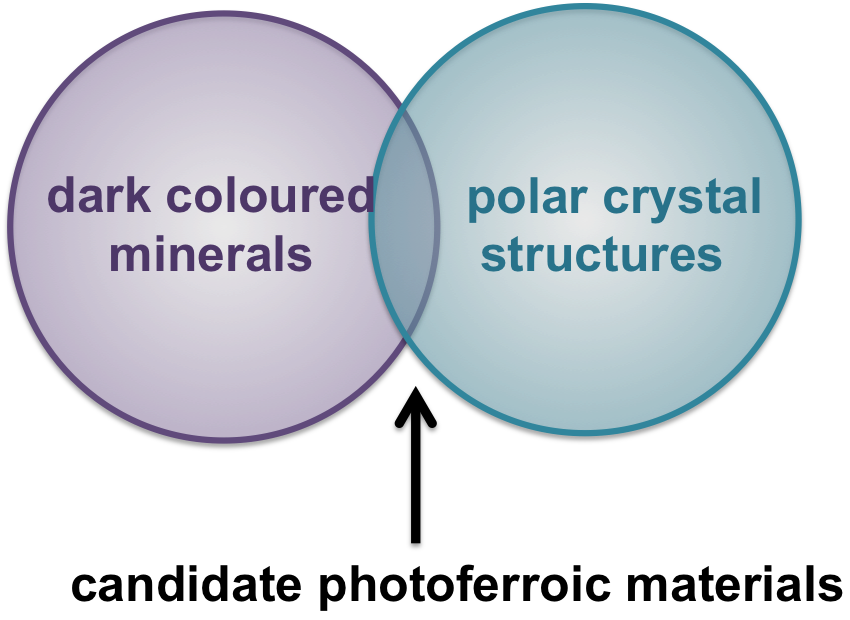
\includegraphics[width=0.5\textwidth]{figures/venn_diagram.png}
    \caption{Venn diagram showing the necessary (but not sufficient) conditions for a material to exhibit photoferroelectricity, where the dark colour suggests absorption of light in the visible range and a polar crystal structure is a requirement (but does not serve as a guarantee) for a material to exhibit ferroelectricity.}
  \label{vd}
\end{figure}

Scientific research on sulfosalts has largely focussed on the thermodynamic properties and crystal structure of the materials, leaving knowledge of the optoelectronic properties of sulfosalts relevant for PV applications extremely scarce. 
The potential of sulfosalt minerals for PV applications however was highlighted by Dittrich et al in 2007 \cite{Dittrich2}. This work also provides an overview of thin film deposition methods that have been developed for sulfosalt layers and discusses a 1\% efficient Sn-Sb-S sulfosalt thin film solar cell constructed by the authors. The thin film deposition methods discussed for other sulfosalt materials would also be particularly important for the eventual aim of constructing PV devices from these materials. The potential of the sulfosalt mineral enargite for PV applications has been suggested even earlier by Pauport\'{e} and Lincot in 1995 \cite{enargite_properties}. In addition to synthesis methods, another important consideration for the large-scale deployment of solar devices composed of the candidate materials is the price and abundance of the elemental components. Figure \ref{abundance} shows a comparison of the price and abundance of some of the elemental components of the three candidate materials: Cu, Sb and S, to that of elements used in some current commercial thin film solar cell absorber materials such as CuIn(Ga)Se$_{2}$ (CIGS) and CdTe. The components of the candidate materials not included in the figure are As, Pb and Ag. Lead can be considered as the most abundant and universally diffused metal after iron. Although it is never found in the native state, its ores are very numerous \cite{abundance}. 5,200,000 tonnes of lead was produced in 2012 \cite{ab_prod}, although its crustal abundance is considerably smaller than that of iron being around 10-14 ppm to compared to approximately 60,000 ppm for iron \cite{ab_1}. 
Silver and arsenic are both fairly abundant metals. Silver often occurs in combination with lead, copper, iron, antimony and tellurium. Arsenic is also present in most ores of silver \cite{abundance}. The crustal abundance of arsenic is approximately 1.5 ppm and that of silver is relatively low at approximately 0.070 ppm \cite{ab_1}. These values are however still larger than that of indium (0.049 ppm \cite{ab_1}), which is also in demand for the display industry \cite{SS}.\\

\begin{figure}[h!]
  \centering
    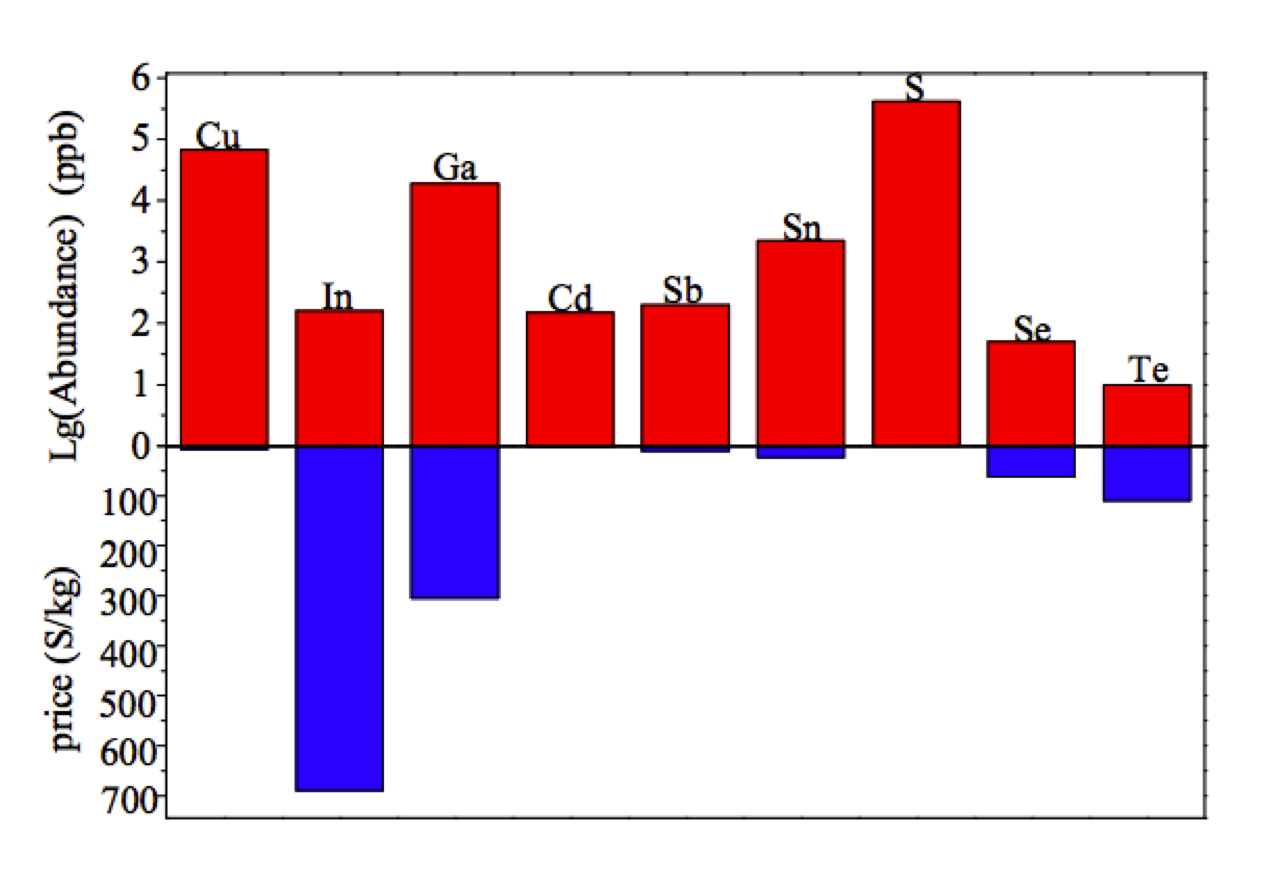
\includegraphics[width=0.7\textwidth]{figures/abundance.png}
    \caption{Comparison of element abundance and price between Cu, In, Ga, Cd, Sb, Sn, S, Se and Te. Figure taken from the supporting information of reference \citenum{Shiyou}, where data was taken from the London Metal Exchange LME.}
  \label{abundance}
\end{figure}

The first candidate photoferroelectric material, enargite (\enargite), is a mineral that corresponds to a semiconductor of type $A^I_3B^VC^{II}_4$, and is frequently found as an impurity in copper ores \cite{enargite_EIS}.
Minerals of the composition $Cu_3(As,Sb)S_4$ are known to occur in two polymorphs: tetragonal with sulfur in cubic close packing or orthorhombic with sulfur in hexagonal close packing. In both cases the coordination is tetrahedral for all atoms \cite{ores}. Enargite is the most common member of this group of minerals, its unit cell (as shown in figure \ref{unit_cells}a) has an orthorhombic crystal structure with space group $Pmn2_1$ and chemical composition \enargite with  a small percentage of Sb \cite{ores1}. The main impurities in natural enargite are Sb and Fe, but Pb and Ag are also known to be present to some extent \cite{enargite_EIS}.
Natural samples of enargite have been found to exhibit the electrical properties of a p-type doped semiconductor with a conductivity of  0.0014 S/m (from the stated value of approximately 7 $\Omega$ cm for the resistivity at 295 K) \cite{enargite_properties}. In the same work, two optical transitions were determined: an indirect one at 1.19 eV and a direct one at 1.44 eV. Although more recent studies have given a value of 1.28 eV for the band gap of enargite from measurements of temperature dependent resistivities, diffuse reflectance spectroscopy and photoacoustic spectroscopy  \cite{Dittrich1}. A theoretical study using the first principles quasi-particle GW method based on wavefunctions generated from the hybrid functional HSE06 \cite{HSE}, has predicted a value of 1.32 eV for the band gap \cite{Zunger}. Although a number of different values have been reported for the band gap of enargite, all values stated fit within the optimal range of 1.06 eV to 1.50 eV \cite{CZTS_book} for a solar absorber material.\\

\begin{figure}[h!]
  \centering
    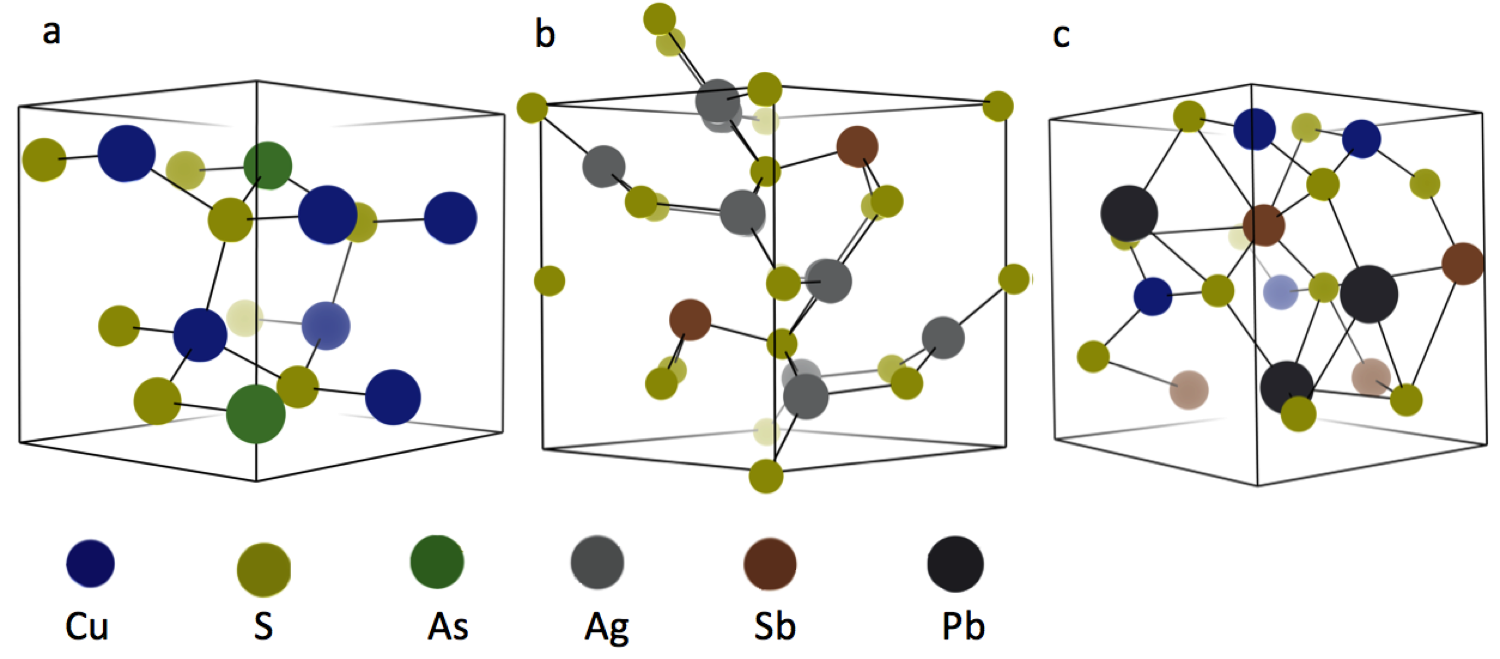
\includegraphics[width=1.0\textwidth]{figures/unit_cells.png}
    \caption{The 15 atom primitive unit cell of enargite (\enargite) (a), 19 atom primitive unit cell of stephanite (\stephanite) (b) and 23 atom primitive unit cell of bournonite (\bournonite) (c).}
  \label{unit_cells}
\end{figure}

The unit cell of the second candidate photoferroelectric material, stephanite (\stephanite), also has an orthorhombic crystal structure but with space group $Cmc2_1$, and is shown in figure \ref{unit_cells}b. 
The structure is composed of columns of $SbS_3$ pyramids extended along the z axis. The columns are located pairwise; in each column, pyramids occupied with antimony atoms alternate with empty pyramids. The Sb-S distances in the pyramids are 2.48, 2.42, and 2.42 $\AA$. Silver atoms are located in the tetrahedral coordination between $SbS_3$ groups (at the centers of rhombic channels). Three types of $AgS_4$ tetrahedra with different Ag-S distances can be identified. The distinctive feature of the structure is a large number of common edges of Ag tetrahedra \cite{stephanite}.
It has been reported that stephanite has a band gap of 1.62 eV \cite{Dittrich1}. Otherwise, there is seemingly very little information available in the literature on the optical or electrical properties of stephanite apart from a work in 1973, given in reference \citenum{stephanite_old}, showing the electrical resistivity of a synthetic sample of stephanite as a function of temperature. The work measures a resistivity of approximately 9 $\Omega$ cm for the stephanite sample at 110 $^\circ$C, which corresponds to a conductivity of 0.0011 S/m. There has also been some speculation in the literature on the possibility of ferroelectric behaviour in stephanite due to the presence of ferroelectric phases at very low temperatures in pyrargyrite ($Ag_3SbS_3$), proustite ($Ag_3AsS_3$) and stibnite ($Sb_2S_3$), which are crystallochemically related to stephanite \cite{stephanite}. The same study also notes that similar displacement structural changes occur in stephanite to those in proustite and pyrargyrite that are responsible for the ferroelectric properties of these materials.\\

Similarly, up until very recently, little information has been available on the optical or electrical properties of the third candidate photoferroelectric material, bournonite (\bournonite). Bournonite also has an orthorhombic crystal structure and the same space group as enargite,  $Pmn2_1$, with measured values of 1.23 eV \cite{Dittrich1} and 1.31 eV \cite{bournonite} reported for the band gap. However, very recently this material has received increasing scientific interest for thermoelectric and rewriteable data storage applications due to a measured low thermal conductivity \cite{Dong}. 
Consequently, works on the synthesis of bournonite are beginning to emerge such as that in reference \citenum{bournonite}.
The low thermal conductivity of bournonite has been attributed to the distortive environment of the Pb and Sb atoms from the stereochemically active lone-pair $s^2$ electrons \cite{Dong}. In the same study they perform electronic structure calculations to predict the band structure of the material, however in the study they use only the generalized-gradient approximation (GGA) level of accuracy in density functional theory for their calculations, which is know to underestimate the band gap of a semiconducting material. They do however show that the inclusion of spin-orbit coupling (SOC) has a considerable impact on the calculated band gap of the material. In the study they predict a direct band gap of 0.686 eV before including SOC and two optical transitions when they do include SOC: a direct band gap of 0.445 eV and an indirect band gap of 0.385 eV. Different levels of accuracy in DFT electronic structure calculations and the impact of SOC on the optoelectronic properties of a material are discussed further in sections \ref{DFT_section} and \ref{SOC_section} respectively. 
A more reason study has made use of DFT+U methodology to avoid the underestimation of the band gap when calculating the optoelectronic properties of this material, where they predicted a band gap of 1.22 eV \cite{bournonite_new}. There was however no mention of SOC in the study, which was shown in the older study to influence to band structure of the material considerably, and the limitations of DFT+U methodology are discussed in section \ref{DFT_section}.\\


\begin{table}[]
\centering
\caption{Summary of known key properties of the three candidate photoferroelectric materials from the literature.}
\label{properties}
\begin{threeparttable}
\begin{tabular}{lllll}
\toprule[1.2pt]
\multicolumn{1}{l}{Candidate} & \multicolumn{1}{l}{Empirical Formula} &  \multicolumn{1}{l}{Space Group} & \multicolumn{1}{l}{Band Gap (eV)} & \multicolumn{1}{l}{Conductivity (S/m)} \\ \midrule[1pt]
Enargite                      &     \enargite         &                                $Pmn2_1$  & 1.28 \cite{Dittrich1}                 & 0.0014 \cite{enargite_properties} \tnote{ii}                           \\
Stephanite                    &   \stephanite &                                $Cmc2_1$ & 1.62  \cite{Dittrich1}                    & 0.0011 \cite{stephanite_old} \tnote{ii}                                    \\
Bournonite                    &      \bournonite  &         $Pmn2_1$                &          1.23 \cite{Dittrich1}, 1.31 \cite{bournonite}                        & -                                     
 \\ \bottomrule[1.2pt]
\end{tabular}
\begin{tablenotes}
\item[i] From resistivity of a natural sample measured at 295 K \item[ii] From resistivity of a synthetic sample measured at 383 K
\end{tablenotes}
\end{threeparttable}
\end{table}

The key known experimentally derived properties of the three candidate materials that were described above are summarised in table \ref{properties}. In this study we aim to use the highest level of theory possible to calculate as many of the properties relevant for a solar absorber material as possible, which were discussed in section \ref{PV_properties}, in order to determine if these materials are likely to perform well in this application. 
Although these materials were originally selected based on the possibility of exhibiting ferroelectricity, for now the study is just focused on the optoelectronic properties that are directly relevant for predicting the performance of these materials in a photovoltaic device. 
Firstly we use hybrid-DFT electronic structure calculations to optimize the crystal structure of a bulk system, starting from the highest quality X-Ray diffraction data available for the materials. From this we calculate the band structures of the materials to determine the size of the band gap and whether it is direct or indirect in nature as this would be a good indicator of how strongly the materials will absorb sunlight. We then go on to calculate the dielectric function and optical absorption coefficients of the materials...\\

%**Emphasize that we identify candidate FE-PV materials, but are currently only assessing their properties to see how well they are likely to perform for PV.


